\section{Holdout results}
\label{sec:final-holdout}

The holdout covers 723 trading days from January 2, 2024 to November 17,
2026. Over this period, factor-hedged Treynor--Black returns TBRETURN
after fees with a Sharpe ratio of TBSHARPE, while PCA pairs earns
PAIRSRETURN with a Sharpe ratio of PAIRSSHARPE. The difference comes from
both trading performance and costs: Treynor--Black generates little profit
before fees and trades frequently, whereas pairs earns more with lower
turnover.

We carry forward the window lengths selected on 2002--2017 and checked on
2018--2023, retaining $K=5$ from the earlier analysis. Each strategy runs with
one fixed configuration:
\begin{itemize}
    \item \textbf{Contrarian, factor-hedged Treynor--Black.} A 60-day
    factor regression, daily refits, and a score cap of three standard
    deviations. Targets are dollar neutral and factor neutral, with unit
    gross exposure.
    \item \textbf{PCA pairs.} A 20-day spread window, 50 disjoint
    loading-based pairs, reselection every 21 days using a 250-day formation
    window, and entry/exit thresholds of 2 and 0.5. Idle allocations remain
    in cash.
\end{itemize}
Both use a 500-day PCA window, five-day PCA refits, and fees of 5 basis
points per dollar traded. Portfolios start in cash, with models initialized
from the final 500 observations of the original sample. As in the earlier
tests, signals include the current day's return and trades execute at that
close.

\subsection{Performance and interpretation}

Table~\ref{tab:final-holdout} reports net performance under the framework's
gap-aware accounting. Pairs achieves a positive Sharpe ratio and a smaller
drawdown, although its annualized return remains modest.

\begin{table}[htbp]
\centering
\small
\begin{tabular}{lrrrr}
\toprule
Strategy & Net return & CAGR & Sharpe & Max DD \\
\midrule
TABLEROWS
\bottomrule
\end{tabular}
\caption{Holdout performance of the selected strategies, with $K=5$ and
5 bp trading fees. CAGR and Sharpe use 252-day annualization and Sharpe uses
a zero risk-free rate. Returns include entry fees but no forced final
liquidation. Cash interest, borrowing costs, slippage, and market impact
are excluded.}
\label{tab:final-holdout}
\end{table}

\paragraph{Treynor--Black: weak gains and high turnover.}
Treynor--Black earns TBPNL of starting capital from trading before paying
TBFEES in fees. At an average daily turnover of TBTURNOVER of equity,
even the 5 bp charge outweighs its trading gains. Those gains are also
uneven: performance before fees is nearly flat in 2024, positive in 2025,
and negative in 2026 through November 17. Reducing costs would help, but
the signal itself does not produce consistent profits in this sample.
Hedging the estimated factors does not resolve that problem, since a
factor-neutral position can still lose money if residual returns fail to
reverse. The results alone cannot tell us whether estimation noise or a
change in the reversal relationship is responsible.

\paragraph{PCA pairs: lower turnover, modest profitability.}
Pairs earns enough before fees to remain profitable in each of the three
calendar years shown, including the partial year in 2026. Its trading gains
contribute PAIRSPNL of starting capital, of which PAIRSFEES is spent on
fees. Average daily turnover is PAIRSTURNOVER, less than half that of
Treynor--Black. The lower trading burden therefore helps preserve a larger
share of its gains.

The positive result is still small in absolute terms. Pairs uses average
gross exposure of PAIRSGROSS, compared with TBGROSS for Treynor--Black,
because inactive pairs leave part of the portfolio in cash. Borrowing costs
and less favorable execution could reduce the remaining profit further.
For both strategies, the trading gains and fees above are additive
contributions from the simulated portfolio, rather than results from a
separate run without costs.

\begin{figure}[htbp]
\centering
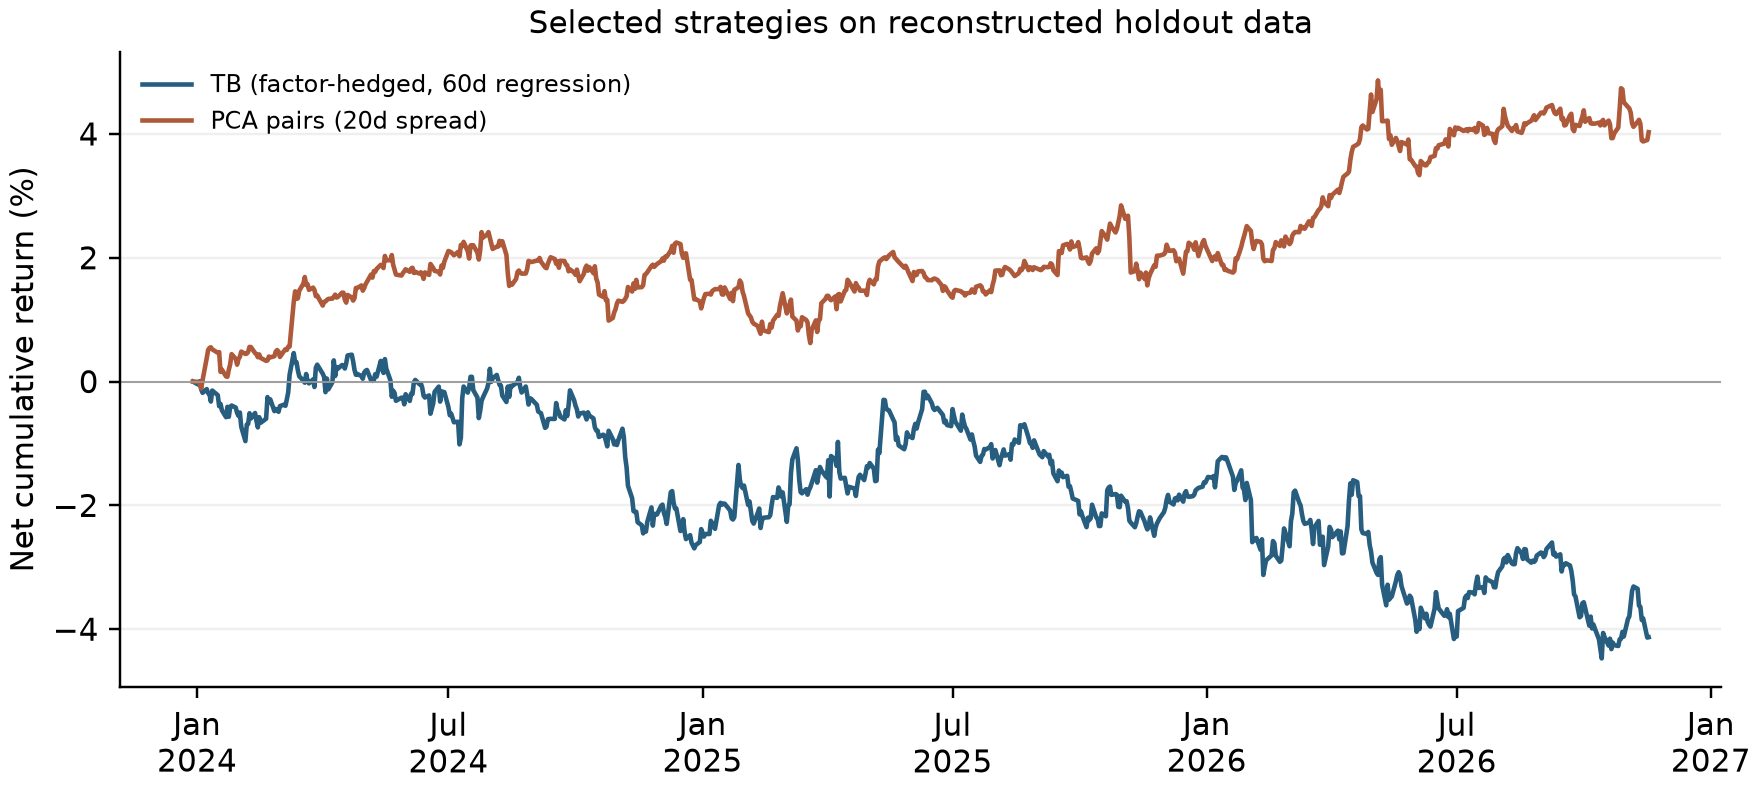
\includegraphics[width=\linewidth]{figures/holdout_performance.png}
\caption{Net cumulative returns for contrarian, factor-hedged Treynor--Black
with a 60-day regression and PCA pairs with a 20-day spread window. Both use
$K=5$ and 5 bp trading fees. Positions start in
cash and begin earning returns after the first holdout close. Missing
observations freeze held positions at their carried marks.}
\label{fig:final-holdout-performance}
\end{figure}

\subsection{Limits of the evaluation}

Missing observations affect how much confidence we can place in these
returns. A stock needs 500 consecutive valid returns to enter estimation.
If its data becomes unavailable while it is held, we keep its dollar mark
unchanged and prohibit trading until observations resume. That capital
remains committed, and the missing interval's return is not recovered.
By the end of the holdout, frozen gross exposure reaches TBENDFROZEN of
equity for Treynor--Black and PAIRSENDFROZEN for pairs. Unknown liquidation
proceeds and terminal payouts could therefore change the results,
particularly for Treynor--Black, while frozen positions can also weaken
portfolio neutrality.

The reported results use corrected data and unchanged strategy parameters.
Earlier runs of this period were inspected before those corrections, so
this evaluation should not be treated as a previously unseen test.

\begin{figure}[htbp]
\centering
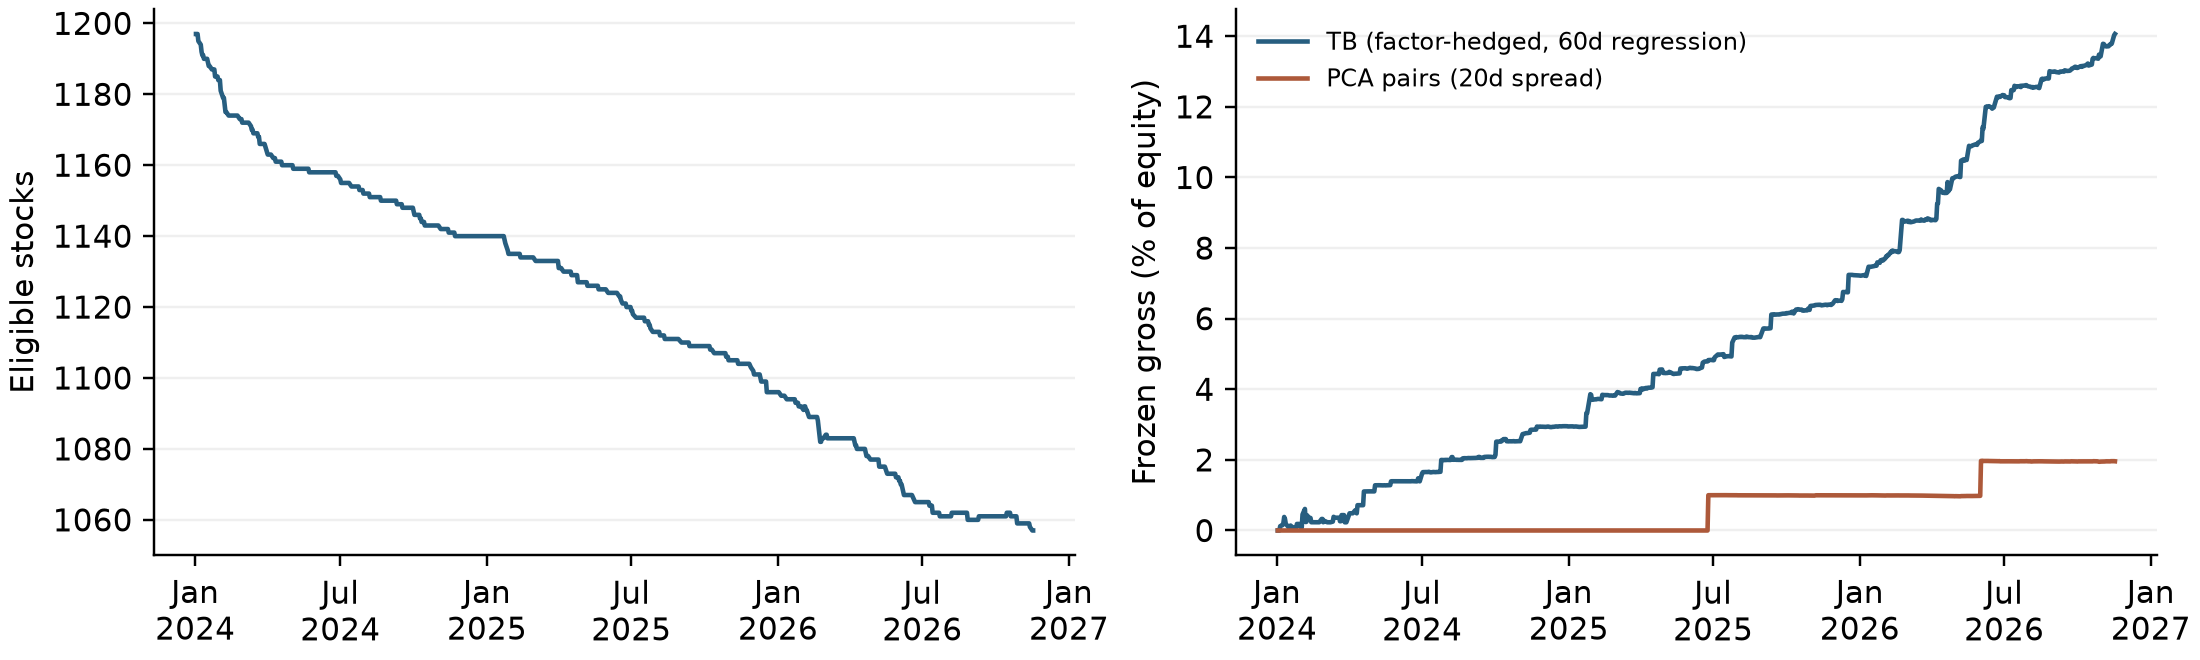
\includegraphics[width=\linewidth]{figures/holdout_data_coverage.png}
\caption{Left: stocks eligible under the trailing 500-day observation rule.
Right: frozen gross exposure as a percentage of current equity for each
selected strategy. Frozen holdings retain their dollar marks while returns
are unavailable, consume portfolio capacity, and may weaken neutrality.
The eligibility rule uses only observations available through each date.}
\label{fig:final-holdout-coverage}
\end{figure}
